% --------------------------- Implementation ---------------------------------

\pagebreak

\section{Implementation}
\subsection{Features From RM}
\noindent
For the initial prototype development, a subset of the requirements from the Requirement Matrix (RM) was carefully selected to focus on implementing core functionalities and demonstrating proof of concept. The selection was based on a combination of high-priority functional requirements that form the backbone of the system, ensuring that critical features are built and validated before expanding the scope.

The requirements chosen for the prototype primarily involve data preprocessing, model training, and evaluation processes. These requirements were selected because they are fundamental to the project's success, ensuring that the data pipeline and model implementation work seamlessly together. This subset of features lays the groundwork for later integration with additional components and more complex functionality.

The filtered part of the RM focuses on the following high-priority requirements: data cleaning and feature extraction, training of machine learning models, and evaluation of model performance using standard metrics. These requirements were identified as crucial because they directly impact the system's ability to handle data, learn patterns, and provide meaningful outputs. Without successfully implementing these core features, the overall effectiveness of the solution would be significantly reduced.

Furthermore, these selected features align with the project’s goals and provide a clear pathway for incremental development. By narrowing down the requirements to these foundational aspects, the development team can ensure that the prototype is not only functional but also extensible, providing a robust framework for future enhancements.

\begin{figure}[h!]  
    \centering
    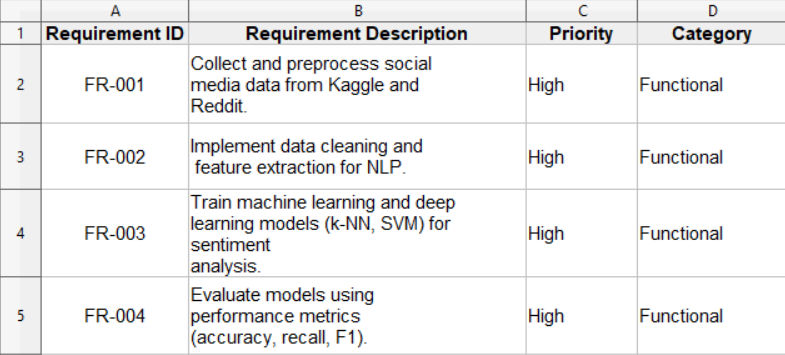
\includegraphics[width=0.7\textwidth]{Images/RM_part_for_implementation.png}  
    \caption{Features from Requirement Matrix}
    \label{Features from Requirement Matrix}  % Label for referencing the figure
\end{figure}

\subsection{Code Details and Output}

\subsubsection{Data Collection}

\begin{tcolorbox}[colback=gray!5!white, colframe=gray!80!black, boxrule=0.5pt, title=Collecting Reddit Posts]
    \begin{lstlisting}[language=Python]
import praw
import pandas as pd
import time
# Initialize Reddit API
reddit = praw.Reddit(client_id='YOUR_CLIENT_ID',
                        client_secret='YOUR_CLIENT_SECRET',
                        user_agent='Mental Health Classifier')
# Define subreddits and post types
subreddits = {'normal': ['news', 'AskReddit'], 
                'depression': ['depression'], 
                'ptsd': ['PTSD'], 
                'anxiety': ['Anxiety'], 
                'bipolar': ['BipolarReddit']}
post_types = ['hot', 'new', 'top']
posts_per_type = 100
# Collect and save posts
data = []
for label, subs in subreddits.items():
    for sub in subs:
        for post_type in post_types:
            posts = getattr(reddit.subreddit(sub), post_type)(limit=posts_per_type)
            for post in posts:
                data.append([post.title + " " + post.selftext, label])
            time.sleep(1)
df = pd.DataFrame(data, columns=['text', 'label'])
df.to_csv(f'{label}_dataset.csv', index=False)
    \end{lstlisting}
    \end{tcolorbox}
    
    \begin{figure}[h!]  
        \centering
        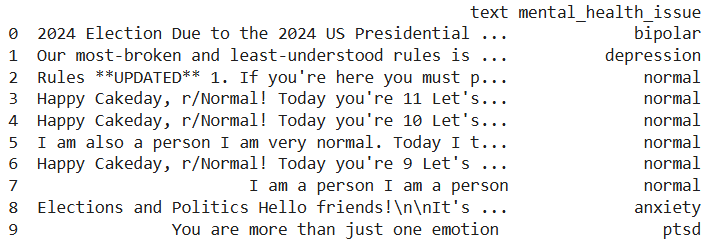
\includegraphics[width=0.9\textwidth]{Images/Dataset.png}  
        \caption{Obtained Dataset}
        \label{LSTMROC711}  % Label for referencing the figure
    \end{figure}


    \begin{tcolorbox}[colback=gray!5!white, colframe=gray!80!black, boxrule=0.5pt, title=Combining Collected Datasets]
    \begin{lstlisting}[language=Python]
    import pandas as pd
    from sklearn.utils import shuffle
    
    # Load datasets
    bipolar_df = pd.read_csv("bipolar_dataset.csv")
    depression_df = pd.read_csv("depression_dataset.csv")
    normal_df = pd.read_csv("normal_dataset.csv")
    anxiety_df = pd.read_csv("anxiety_dataset.csv")
    ptsd_df = pd.read_csv("ptsd_dataset.csv")
    
    # Minimum length for balanced classes
    min_length = min(len(bipolar_df), len(depression_df), len(normal_df) // 6, len(anxiety_df), len(ptsd_df))
    
    # Create balanced pattern
    pattern_data = []
    for i in range(min_length):
        pattern_data.extend([bipolar_df.iloc[i], depression_df.iloc[i]] +
                            normal_df.iloc[i*6:(i+1)*6].to_dict('records') +
                            [anxiety_df.iloc[i], ptsd_df.iloc[i]])
    
    pattern_df = pd.DataFrame(pattern_data)
    remaining_data = shuffle(pd.concat([bipolar_df[min_length:], depression_df[min_length:], 
                                        normal_df[min_length*6:], anxiety_df[min_length:], ptsd_df[min_length:]]))
    
    final_df = pd.concat([pattern_df, remaining_data]).reset_index(drop=True)
    final_df.to_csv("mental_health_combined.csv", index=False)
    \end{lstlisting}
    \end{tcolorbox}
    
    \noindent
    The first code snippet collects Reddit posts by connecting to specific subreddits associated with various mental health topics. Using the Reddit API, posts are retrieved from `hot`, `new`, and `top` categories for each mental health type, including general subreddits (for the "normal" category). Each post’s title and content are combined, labeled, and saved into separate CSV files. The second code snippet merges these CSV files to form a combined dataset. It creates a balanced sample by selecting the minimum number of rows across each category and organizes the data in a structured pattern. Remaining rows are shuffled and appended, producing a final dataset suitable for machine learning applications in mental health classification.
    

    \subsubsection{Data Preprocessing}

    \begin{tcolorbox}[colback=gray!5!white, colframe=gray!80!black, boxrule=0.5pt, title=Text Preprocessing]
        \begin{lstlisting}[language=Python]
        import pandas as pd
        import re
        from sklearn.feature_extraction.text import TfidfVectorizer
        from nltk.corpus import stopwords
        from nltk.tokenize import word_tokenize
        import nltk
    
        # Download stopwords (if you haven't already)
        nltk.download('stopwords')
        nltk.download('punkt')
    
        # Load the dataset
        df = pd.read_csv('mental_health.csv')
    
        # 1. Handling Missing Values
        df.dropna(subset=['text'], inplace=True)
    
        # 2. Removing duplicates (if any)
        df.drop_duplicates(subset=['text'], inplace=True)
    
        # 3. Text Preprocessing
        negative_words = {"not", "no", "nor", "never", "nothing", "nowhere", "neither", "cannot", "n't", "without", "barely", "hardly", "scarcely"}
    
        def clean_text(text):
            text = re.sub(r'http\S+', '', text)  # Remove URLs
            text = re.sub(r'@\w+', '', text)  # Remove mentions (@username)
            text = re.sub(r'[^a-zA-Z\s]', '', text)  # Remove special characters, numbers, and punctuations
            text = text.lower()  # Convert text to lowercase
            tokens = word_tokenize(text)  # Tokenize the text
            tokens = [word for word in tokens if word not in stopwords.words('english') or word in negative_words]  # Remove stopwords, but keep negative words
            clean_text = ' '.join(tokens)  # Join the tokens back into a single string
            return clean_text
    
        df['cleaned_text'] = df['text'].apply(clean_text)  # Apply the cleaning function to the 'text' column
    
    \end{lstlisting}
    \end{tcolorbox}

    \begin{tcolorbox}[colback=gray!5!white, colframe=gray!80!black, boxrule=0.5pt, title=Text Preprocessing]
    \begin{lstlisting}[language=Python]
        # 4. Feature Extraction using TF-IDF Vectorization
        vectorizer = TfidfVectorizer(max_features=10000)  # Adjust the max_features
        X = vectorizer.fit_transform(df['cleaned_text'])  # Fit and transform the cleaned text data
        X_df = pd.DataFrame(X.toarray(), columns=vectorizer.get_feature_names_out())  # Convert the result to a DataFrame for easier understanding
    
        # Save the preprocessed dataset (optional)
        df.to_csv('preprocessed_mental_health.csv', index=False)
        \end{lstlisting}
    \end{tcolorbox}
    
    \noindent
    The code snippet above demonstrates the preprocessing steps for a mental health dataset. It handles missing values and duplicates in the text data, performs text cleaning by removing URLs, mentions, and special characters, and applies tokenization. The cleaned text is then vectorized using TF-IDF to convert the textual data into a format suitable for machine learning models. Finally, the preprocessed dataset is saved as a new CSV file for future use in classification tasks.
    
    \begin{figure}[h!]  
        \centering
        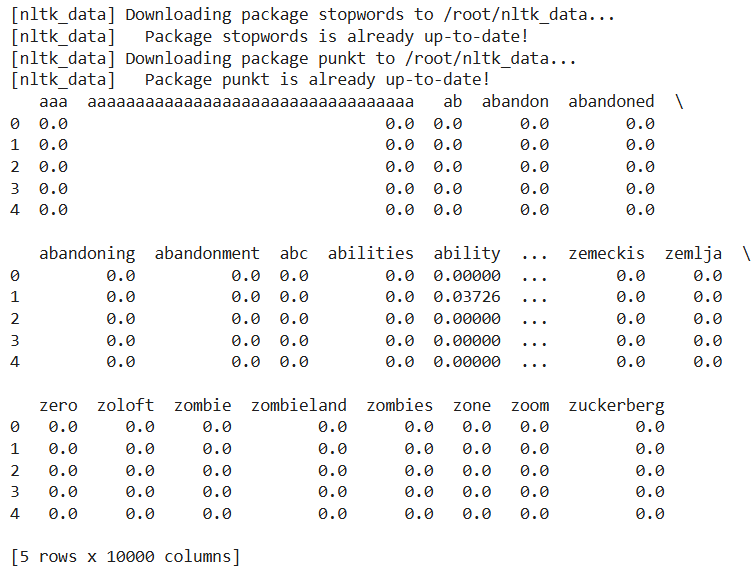
\includegraphics[width=0.9\textwidth]{Images/Data Cleaning and Preprocessing.png}  
        \caption{Data Collection and Preprocessing}
        \label{Data Collection and Preprocessing}  % Label for referencing the figure
    \end{figure}

\subsubsection{Logistic Regression Model for Classification}

\begin{tcolorbox}[colback=gray!5!white, colframe=gray!80!black, boxrule=0.5pt, title=Logistic Regression for Mental Health Classification]
    \begin{lstlisting}[language=Python]
    import pandas as pd
    from sklearn.model_selection import train_test_split
    from sklearn.feature_extraction.text import CountVectorizer
    from sklearn.linear_model import LogisticRegression
    from sklearn.metrics import accuracy_score, classification_report, confusion_matrix

    # Load the preprocessed dataset
    dataset = pd.read_csv('preprocessed_mental_health.csv')

    # Check if 'cleaned_text' and 'mental_health_issue' columns exist
    if 'cleaned_text' not in dataset.columns or 'mental_health_issue' not in dataset.columns:
        raise ValueError("The dataset must have 'cleaned_text' and 'mental_health_issue' columns.")

    # Remove rows with missing values in 'cleaned_text' column
    dataset.dropna(subset=['cleaned_text'], inplace=True)

    # Initialize the CountVectorizer and fit/transform the cleaned text
    LRvectorizer = CountVectorizer()
    X = LRvectorizer.fit_transform(dataset['cleaned_text'])

    # Prepare the target variable
    y = dataset['mental_health_issue']

    # Split the dataset into Training and Test Sets
    X_train, X_test, y_train, y_test = train_test_split(X, y, test_size=0.2, random_state=42)

    # Initialize the Logistic Regression model
    LRmodel = LogisticRegression(multi_class='ovr', max_iter=10000)

    # Train the model
    LRmodel.fit(X_train, y_train)

    # Make predictions on the test set
    y_pred = LRmodel.predict(X_test)

\end{lstlisting}
\end{tcolorbox}

\begin{tcolorbox}[colback=gray!5!white, colframe=gray!80!black, boxrule=0.5pt, title=Logistic Regression for Mental Health Classification]
    \begin{lstlisting}[language=Python]
    # Evaluate the model
    accuracy = accuracy_score(y_test, y_pred)
    print(f'Accuracy: {accuracy * 100:.2f}%')

    # Print classification report
    print("Classification Report:\n", classification_report(y_test, y_pred))

    # Print confusion matrix
    print("Confusion Matrix:\n", confusion_matrix(y_test, y_pred))
    \end{lstlisting}
\end{tcolorbox}

\noindent
The provided code demonstrates how to apply Logistic Regression for mental health classification using a preprocessed dataset. First, the dataset is loaded, and a check is performed to ensure that it contains the necessary columns, specifically \texttt{cleaned\_text} and \texttt{mental\_health\_issue}. If these columns are missing, an error is raised. The dataset is then cleaned by removing rows that have missing values in the \texttt{cleaned\_text} column using the \texttt{dropna()} function. Next, the \texttt{CountVectorizer} is initialized and applied to the \texttt{cleaned\_text} column to convert the text data into a numerical format suitable for machine learning. This is accomplished by transforming the text into a document-term matrix where each row represents a document (post) and each column represents a unique term (word). The target variable, \texttt{mental\_health\_issue}, is also extracted from the dataset.The dataset is then split into training and testing sets using \texttt{train\_test\_split()}, where 80\% of the data is used for training, and 20\% is reserved for testing. The \texttt{random\_state} is set to ensure reproducibility of the results. A Logistic Regression model is initialized with a multi-class strategy (\texttt{multi\_class='ovr'}) and a high number of iterations (\texttt{max\_iter=10000}) to allow the model to converge. The model is then trained on the training data using the \texttt{fit()} method. After training, predictions are made on the test set using the \texttt{predict()} method. The model's performance is evaluated by calculating the accuracy score, which is printed as a percentage. Additionally, a detailed classification report is generated, which includes metrics such as precision, recall, and F1-score for each class. Lastly, a confusion matrix is printed to visualize the model's classification performance and to understand how well the model distinguishes between different mental health issues. This end-to-end pipeline is crucial for applying Logistic Regression to textual data, allowing for effective classification of mental health issues based on Reddit posts.


\subsubsection{Naive Bayes for Classification}

\begin{tcolorbox}[colback=gray!5!white, colframe=gray!80!black, boxrule=0.5pt, title=Naive Bayes for Mental Health Classification]
    \begin{lstlisting}[language=Python]

        import pandas as pd
        from sklearn.model_selection import train_test_split
        from sklearn.feature_extraction.text import CountVectorizer
        from sklearn.naive_bayes import MultinomialNB
        from sklearn.metrics import accuracy_score, classification_report, confusion_matrix
        
        # Load the preprocessed dataset
        dataset = pd.read_csv('preprocessed_mental_health.csv')
        
        # Check if 'cleaned_text' and 'mental_health_issue' columns exist
        if 'cleaned_text' not in dataset.columns or 'mental_health_issue' not in dataset.columns:
            raise ValueError("The dataset must have 'cleaned_text' and 'mental_health_issue' columns.")
        
        # Remove rows with missing values in 'cleaned_text' column
        dataset.dropna(subset=['cleaned_text'], inplace=True)
        
        # Initialize the CountVectorizer and fit/transform the cleaned text
        NBvectorizer = CountVectorizer()
        X = NBvectorizer.fit_transform(dataset['cleaned_text'])
        
        # Prepare the target variable
        y = dataset['mental_health_issue']
        
        # Split the dataset into Training and Test Sets
        X_train, X_test, y_train, y_test = train_test_split(X, y, test_size=0.2, random_state=42)
        
        # Initialize the Naive Bayes classifier
        NBmodel = MultinomialNB()
        
        # Fit the model
        NBmodel.fit(X_train, y_train)
    \end{lstlisting}
\end{tcolorbox}

\begin{tcolorbox}[colback=gray!5!white, colframe=gray!80!black, boxrule=0.5pt, title=Naive Bayes for Mental Health Classification]
    \begin{lstlisting}[language=Python]
        # Make predictions
        y_pred = NBmodel.predict(X_test)
        
        # Evaluate the model
        accuracy = accuracy_score(y_test, y_pred)
        print(f'Accuracy: {accuracy * 100:.2f}%')
        
        # Print classification report
        print("Classification Report:\n", classification_report(y_test, y_pred))
        
        # Print confusion matrix
        print("Confusion Matrix:\n", confusion_matrix(y_test, y_pred))

    \end{lstlisting}
\end{tcolorbox}

\noindent
The provided code demonstrates how to apply the Naive Bayes classifier (MultinomialNB) for mental health classification using a preprocessed dataset. First, the dataset is loaded, and a check is performed to ensure that it contains the necessary columns, specifically \texttt{cleaned\_text} and \texttt{mental\_health\_issue}. If these columns are missing, an error is raised. The dataset is then cleaned by removing rows that have missing values in the \texttt{cleaned\_text} column using the \texttt{dropna()} function. Next, the \texttt{CountVectorizer} is initialized and applied to the \texttt{cleaned\_text} column to convert the text data into a numerical format suitable for machine learning. This is accomplished by transforming the text into a document-term matrix where each row represents a document (post) and each column represents a unique term (word). The target variable, \texttt{mental\_health\_issue}, is also extracted from the dataset. The dataset is then split into training and testing sets using \texttt{train\_test\_split()}, where 80\% of the data is used for training, and 20\% is reserved for testing. The \texttt{random\_state} is set to ensure reproducibility of the results. A Naive Bayes model (\texttt{MultinomialNB}) is initialized and trained on the training data using the \texttt{fit()} method. After training, predictions are made on the test set using the \texttt{predict()} method. The model's performance is evaluated by calculating the accuracy score, which is printed as a percentage. Additionally, a detailed classification report is generated, which includes metrics such as precision, recall, and F1-score for each class. Lastly, a confusion matrix is printed to visualize the model's classification performance and to understand how well the model distinguishes between different mental health issues. This end-to-end pipeline is crucial for applying the Naive Bayes algorithm to textual data, allowing for effective classification of mental health issues based on Reddit posts.

\subsubsection{Support Vector Machine for Classification}

\begin{tcolorbox}[colback=gray!5!white, colframe=gray!80!black, boxrule=0.5pt, title=Support Vector Classifier Implementation]
    \begin{lstlisting}[language=Python]
    import pandas as pd
    from sklearn.model_selection import train_test_split
    from sklearn.feature_extraction.text import CountVectorizer
    from sklearn.svm import SVC
    from sklearn.metrics import accuracy_score, classification_report, confusion_matrix

    # Load the preprocessed dataset
    dataset = pd.read_csv('preprocessed_mental_health.csv')

    # Check if 'cleaned_text' and 'mental_health_issue' columns exist
    if 'cleaned_text' not in dataset.columns or 'mental_health_issue' not in dataset.columns:
        raise ValueError("The dataset must have 'cleaned_text' and 'mental_health_issue' columns.")

    # Remove rows with missing values in 'cleaned_text' column
    dataset.dropna(subset=['cleaned_text'], inplace=True)

    # Initialize the CountVectorizer and fit/transform the cleaned text
    SVMvectorizer = CountVectorizer()
    X = SVMvectorizer.fit_transform(dataset['cleaned_text'])

    # Prepare the target variable
    y = dataset['mental_health_issue']

    # Split the dataset into Training and Test Sets
    X_train, X_test, y_train, y_test = train_test_split(X, y, test_size=0.2, random_state=42)

    # Initialize the Support Vector Classifier
    SVMmodel = SVC(kernel='linear', C=1, random_state=42, probability=True)  # You can adjust parameters as needed

    # Train the model
    SVMmodel.fit(X_train, y_train)

    # Make predictions on the test set
    y_pred = SVMmodel.predict(X_test)
\end{lstlisting}
\end{tcolorbox}

\begin{tcolorbox}[colback=gray!5!white, colframe=gray!80!black, boxrule=0.5pt, title=Support Vector Classifier Implementation]
    \begin{lstlisting}[language=Python]
    # Evaluate the model
    accuracy = accuracy_score(y_test, y_pred)
    print(f'Accuracy: {accuracy * 100:.2f}%')

    # Print classification report
    print("Classification Report:\n", classification_report(y_test, y_pred))

    # Print confusion matrix
    print("Confusion Matrix:\n", confusion_matrix(y_test, y_pred))
    \end{lstlisting}
\end{tcolorbox}

\noindent
The provided code demonstrates how to apply the Support Vector Classifier (SVC) for mental health classification using a preprocessed dataset. First, the dataset is loaded, and a check is performed to ensure that it contains the necessary columns, specifically \texttt{cleaned\_text} and \texttt{mental\_health\_issue}. If these columns are missing, an error is raised. The dataset is then cleaned by removing rows that have missing values in the \texttt{cleaned\_text} column using the \texttt{dropna()} function.Next, the \texttt{CountVectorizer} is initialized and applied to the \texttt{cleaned\_text} column to convert the text data into a numerical format suitable for machine learning. This is accomplished by transforming the text into a document-term matrix where each row represents a document (post) and each column represents a unique term (word). The target variable, \texttt{mental\_health\_issue}, is also extracted from the dataset. The dataset is then split into training and testing sets using \texttt{train\_test\_split()}, where 80\% of the data is used for training, and 20\% is reserved for testing. The \texttt{random\_state} is set to ensure reproducibility of the results. A Support Vector Classifier model (\texttt{SVC}) is initialized with a linear kernel (\texttt{kernel='linear'}), regularization parameter \texttt{C=1}, and the probability flag set to \texttt{True} to enable probability estimates. The model is then trained on the training data using the \texttt{fit()} method. After training, predictions are made on the test set using the \texttt{predict()} method. The model's performance is evaluated by calculating the accuracy score, which is printed as a percentage. Additionally, a detailed classification report is generated, which includes metrics such as precision, recall, and F1-score for each class. Lastly, a confusion matrix is printed to visualize the model's classification performance and to understand how well the model distinguishes between different mental health issues. This end-to-end pipeline is crucial for applying the Support Vector Machine (SVM) algorithm to textual data, allowing for effective classification of mental health issues based on Reddit posts.

\subsubsection{Random Forest for Classification}

\begin{tcolorbox}[colback=gray!5!white, colframe=gray!80!black, boxrule=0.5pt, title=Random Forest Classifier Implementation]
    \begin{lstlisting}[language=Python]
    import pandas as pd
    from sklearn.model_selection import train_test_split
    from sklearn.feature_extraction.text import CountVectorizer
    from sklearn.ensemble import RandomForestClassifier
    from sklearn.metrics import accuracy_score, classification_report, confusion_matrix

    # Load the preprocessed dataset
    dataset = pd.read_csv('preprocessed_mental_health.csv')

    # Check if 'cleaned_text' and 'mental_health_issue' columns exist
    if 'cleaned_text' not in dataset.columns or 'mental_health_issue' not in dataset.columns:
        raise ValueError("The dataset must have 'cleaned_text' and 'mental_health_issue' columns.")

    # Remove rows with missing values in 'cleaned_text' column
    dataset.dropna(subset=['cleaned_text'], inplace=True)

    # Initialize the CountVectorizer and fit/transform the cleaned text
    RFvectorizer = CountVectorizer()
    X = RFvectorizer.fit_transform(dataset['cleaned_text'])

    # Prepare the target variable
    y = dataset['mental_health_issue']

    # Split the dataset into Training and Test Sets
    X_train, X_test, y_train, y_test = train_test_split(X, y, test_size=0.2, random_state=42)

    # Initialize the Random Forest Classifier with added parameters
    RFmodel = RandomForestClassifier(
        n_estimators=3000,         # Number of trees
        max_depth=None,            # Maximum depth of each tree
        min_samples_split=20,      # Minimum number of samples to split a node

\end{lstlisting}
\end{tcolorbox}

\begin{tcolorbox}[colback=gray!5!white, colframe=gray!80!black, boxrule=0.5pt, title=Random Forest Classifier Implementation]
    \begin{lstlisting}[language=Python]
        min_samples_leaf=1,        # Minimum number of samples in a leaf node
        max_features='sqrt',       # Number of features to consider at each split
        bootstrap=False,            # Whether to use bootstrapping

        random_state=42            # For reproducibility
    )

    # Train the model
    RFmodel.fit(X_train, y_train)

    # Make predictions on the test set
    y_pred = RFmodel.predict(X_test)

    # Evaluate the model
    accuracy = accuracy_score(y_test, y_pred)
    print(f'Accuracy: {accuracy * 100:.2f}%')

    # Print classification report
    print("Classification Report:\n", classification_report(y_test, y_pred))

    # Print confusion matrix
    print("Confusion Matrix:\n", confusion_matrix(y_test, y_pred))
    \end{lstlisting}
\end{tcolorbox}

\noindent
The provided code demonstrates how to apply the Random Forest Classifier for mental health classification using a preprocessed dataset. First, the dataset is loaded, and a check is performed to ensure that it contains the necessary columns, specifically \texttt{cleaned\_text} and \texttt{mental\_health\_issue}. If these columns are missing, an error is raised. The dataset is then cleaned by removing rows that have missing values in the \texttt{cleaned\_text} column using the \texttt{dropna()} function. Next, the \texttt{CountVectorizer} is initialized and applied to the \texttt{cleaned\_text} column to convert the text data into a numerical format suitable for machine learning. This is accomplished by transforming the text into a document-term matrix where each row represents a document (post) and each column represents a unique term (word). The target variable, \texttt{mental\_health\_issue}, is also extracted from the dataset. The dataset is then split into training and testing sets using \texttt{train\_test\_split()}, where 80\% of the data is used for training, and 20\% is reserved for testing. The \texttt{random\_state} is set to ensure reproducibility of the results. A Random Forest Classifier model is initialized with several hyperparameters. Specifically, \texttt{n\_estimators=3000} defines the number of decision trees in the forest. The \texttt{max\_depth=None} means the trees are allowed to grow until all leaves are pure or contain fewer than the minimum samples required to split a node. The \texttt{min\_samples\_split=20} and \texttt{min\_samples\_leaf=1} specify the minimum number of samples required to split an internal node and the minimum number of samples required to be at a leaf node, respectively. The \texttt{max\_features='sqrt'} sets the maximum number of features to consider for the best split at each node to be the square root of the total number of features. \texttt{bootstrap=False} disables bootstrapping, meaning the entire dataset is used to build each tree. After initialization, the model is trained using the \texttt{fit()} method on the training data. After training, predictions are made on the test set using the \texttt{predict()} method. The model's performance is evaluated by calculating the accuracy score, which is printed as a percentage. Additionally, a detailed classification report is generated, which includes metrics such as precision, recall, and F1-score for each class. Lastly, a confusion matrix is printed to visualize the model's classification performance and to understand how well the model distinguishes between different mental health issues. This end-to-end pipeline is essential for applying the Random Forest algorithm to textual data, allowing for effective classification of mental health issues based on Reddit posts.

\subsubsection{XGBoost for Classification}

\begin{tcolorbox}[colback=gray!5!white, colframe=gray!80!black, boxrule=0.5pt, title=XGBoost Classifier Implementation]
    \begin{lstlisting}[language=Python]
    import pandas as pd
    from sklearn.model_selection import train_test_split
    from sklearn.preprocessing import LabelEncoder
    from sklearn.metrics import accuracy_score, classification_report, confusion_matrix
    import xgboost as xgb

    # Load the dataset
    data = pd.read_csv('preprocessed_mental_health.csv')

    # Separate features and target
    X = data['text']
    y = data['mental_health_issue']

    # Encode target labels
    label_encoder = LabelEncoder()
    y = label_encoder.fit_transform(y)

    # Split dataset into training and test sets
    X_train, X_test, y_train, y_test = train_test_split(X, y, test_size=0.2, random_state=42)

\end{lstlisting}
\end{tcolorbox}

\begin{tcolorbox}[colback=gray!5!white, colframe=gray!80!black, boxrule=0.5pt, title=XGBoost Classifier Implementation]
    \begin{lstlisting}[language=Python]
    # Convert text data to numerical data using TF-IDF Vectorizer
    from sklearn.feature_extraction.text import TfidfVectorizer
    tfidf = TfidfVectorizer(max_features=5000)
    X_train = tfidf.fit_transform(X_train)
    X_test = tfidf.transform(X_test)

    # Define the XGBoost classifier
    xgb_clf = xgb.XGBClassifier(objective='multi:softmax', num_class=5, eval_metric='mlogloss', use_label_encoder=False)

    # Train the model
    xgb_clf.fit(X_train, y_train)

    # Predict on the test set
    y_pred = xgb_clf.predict(X_test)

    # Evaluate the model
    accuracy = accuracy_score(y_test, y_pred)
    report = classification_report(y_test, y_pred, target_names=label_encoder.classes_)

    print(f"Accuracy: {accuracy * 100:.2f}%")
    print("Classification Report:\n", report)

    # Print confusion matrix
    print("Confusion Matrix:\n", confusion_matrix(y_test, y_pred))
    \end{lstlisting}
\end{tcolorbox}

\noindent
The provided code demonstrates how to apply XGBoost for mental health classification using a preprocessed dataset. First, the dataset is loaded, and the target variable (\texttt{mental\_health\_issue}) is separated from the feature variable (\texttt{text}). The target variable is then encoded using \texttt{LabelEncoder()} to convert the categorical labels into numerical values, which are required for machine learning algorithms. Next, the dataset is split into training and testing sets using \texttt{train\_test\_split()}, where 80\% of the data is used for training, and 20\% is reserved for testing. The \texttt{random\_state} is set to ensure reproducibility of the results. The text data is then transformed into numerical features using the \texttt{TfidfVectorizer()}. This vectorizer converts the raw text into a matrix of TF-IDF (Term Frequency-Inverse Document Frequency) features, which are more suitable for training a machine learning model. The \texttt{max\_features=5000} parameter limits the number of features to the 5000 most frequent terms in the dataset. The XGBoost classifier is then initialized with several hyperparameters. The \texttt{objective='multi:softmax'} indicates that the task is a multi-class classification problem. The \texttt{num\_class=5} parameter specifies the number of classes for the classification task, and \texttt{eval\_metric='mlogloss'} is set to use the log loss metric for evaluation. \texttt{use\_label\_encoder=False} disables the automatic label encoding of target labels, as we have already manually encoded the labels. After initialization, the model is trained on the training data using the \texttt{fit()} method. After training, predictions are made on the test set using the \texttt{predict()} method. The model's performance is evaluated by calculating the accuracy score, which is printed as a percentage. Additionally, a detailed classification report is generated, which includes metrics such as precision, recall, and F1-score for each class. Lastly, a confusion matrix is printed to visualize the model's classification performance and to understand how well the model distinguishes between different mental health issues. This pipeline demonstrates the use of XGBoost in combination with TF-IDF vectorization for text classification, enabling effective classification of mental health issues based on Reddit posts.


\subsubsection{K Nearest Neighbours for Classification}

\begin{tcolorbox}[colback=gray!5!white, colframe=gray!80!black, boxrule=0.5pt, title=k-NN Classifier Implementation for Mental Health Classification]
    \begin{lstlisting}[language=Python]
import pandas as pd
from sklearn.model_selection import train_test_split
from sklearn.feature_extraction.text import CountVectorizer
from sklearn.neighbors import KNeighborsClassifier
from sklearn.metrics import accuracy_score, classification_report, confusion_matrix

# Load the preprocessed dataset
dataset = pd.read_csv('preprocessed_mental_health.csv')

# Check if 'cleaned_text' and 'mental_health_issue' columns exist
if 'cleaned_text' not in dataset.columns or 'mental_health_issue' not in dataset.columns:
    raise ValueError("The dataset must have 'cleaned_text' and 'mental_health_issue' columns.")

# Remove rows with missing values in 'cleaned_text' column
dataset.dropna(subset=['cleaned_text'], inplace=True)

# Initialize the CountVectorizer and fit/transform the cleaned text
KNNvectorizer = CountVectorizer()
X = KNNvectorizer.fit_transform(dataset['cleaned_text'])
\end{lstlisting}
\end{tcolorbox}

\begin{tcolorbox}[colback=gray!5!white, colframe=gray!80!black, boxrule=0.5pt, title=k-NN Classifier Implementation for Mental Health Classification]
    \begin{lstlisting}[language=Python]
# Prepare the target variable
y = dataset['mental_health_issue']

# Split the dataset into Training and Test Sets
X_train, X_test, y_train, y_test = train_test_split(X, y, test_size=0.2, random_state=42)

# Initialize the k-NN classifier
KNNmodel = KNeighborsClassifier(n_neighbors=5)  # You can adjust the number of neighbors

# Fit the model
KNNmodel.fit(X_train, y_train)

# Make predictions
y_pred = KNNmodel.predict(X_test)

# Evaluate the model
accuracy = accuracy_score(y_test, y_pred)
print(f'Accuracy: {accuracy * 100:.2f}%')

# Print classification report
print("Classification Report:\n", classification_report(y_test, y_pred))

# Print confusion matrix
print("Confusion Matrix:\n", confusion_matrix(y_test, y_pred))
    \end{lstlisting}
\end{tcolorbox}

\noindent
The code provided demonstrates how to implement a k-Nearest Neighbors (k-NN) classifier for mental health issue classification based on text data. Initially, the dataset is loaded from a CSV file, and a check is performed to ensure the presence of the necessary columns, namely \texttt{cleaned\_text} and \texttt{mental\_health\_issue}. If any of these columns are missing, the program raises an error. The next step involves removing rows with missing text data from the \texttt{cleaned\_text} column using \texttt{dropna()}. The \texttt{CountVectorizer} from \texttt{sklearn} is used to transform the textual data into a matrix of token counts, which is suitable for machine learning. This transformation converts each post (document) into a vector of word occurrences, with each unique word in the dataset being represented by a column. The target variable, \texttt{mental\_health\_issue}, is extracted, and the dataset is split into training and test sets using \texttt{train\_test\_split()}. The training set consists of 80\% of the data, and the remaining 20\% is used for testing. A k-NN classifier is initialized with 5 neighbors (\texttt{n\_neighbors=5}), though this number can be adjusted for tuning the model. The classifier is trained on the training data using the \texttt{fit()} method. Once the model is trained, it is used to predict mental health issues for the test set, and the accuracy of the predictions is calculated and printed. In addition to the accuracy score, a detailed classification report is generated, which includes metrics like precision, recall, and F1-score for each class. Finally, a confusion matrix is printed to help visualize the model’s performance in terms of how well it classifies different mental health issues. This end-to-end pipeline demonstrates how to apply a k-NN classifier to a text classification task, specifically identifying mental health issues based on user-generated content such as social media posts.




\subsubsection{Long Short Term Memory based Classification}

\begin{tcolorbox}[colback=gray!5!white, colframe=gray!80!black, boxrule=0.5pt, title=LSTM Model Implementation]
    \begin{lstlisting}[language=Python]
    import pandas as pd
    import numpy as np
    import matplotlib.pyplot as plt
    import seaborn as sns
    from sklearn.metrics import confusion_matrix, classification_report
    from sklearn.preprocessing import LabelEncoder
    from tensorflow.keras.preprocessing.text import Tokenizer
    from tensorflow.keras.preprocessing.sequence import pad_sequences
    from tensorflow.keras.models import Sequential
    from tensorflow.keras.layers import Embedding, LSTM, Dense, Dropout
    from tensorflow.keras.utils import to_categorical
    from sklearn.model_selection import train_test_split

    # Load the dataset
    data = pd.read_csv('preprocessed_mental_health.csv')

    # Separate features and target
    X = data['text']
    y = data['mental_health_issue']

    # Encode target labels
    label_encoder = LabelEncoder()
    y = label_encoder.fit_transform(y)
    y = to_categorical(y)  # Convert labels to one-hot encoded format for multi-class classification

    # Split dataset into training and test sets
    X_train, X_test, y_train, y_test = train_test_split(X, y, test_size=0.2, random_state=42)
\end{lstlisting}
\end{tcolorbox}

\begin{tcolorbox}[colback=gray!5!white, colframe=gray!80!black, boxrule=0.5pt, title=LSTM Model Implementation]
    \begin{lstlisting}[language=Python]
    # Tokenize and pad the text sequences
    vocab_size = 10000  # Set a vocabulary size
    max_length = 100    # Set a max length for padding

    tokenizer = Tokenizer(num_words=vocab_size, oov_token="<OOV>")
    tokenizer.fit_on_texts(X_train)

    X_train_seq = tokenizer.texts_to_sequences(X_train)
    X_test_seq = tokenizer.texts_to_sequences(X_test)

    X_train_padded = pad_sequences(X_train_seq, maxlen=max_length, padding='post', truncating='post')
    X_test_padded = pad_sequences(X_test_seq, maxlen=max_length, padding='post', truncating='post')

    # Build the LSTM model
    model = Sequential([
        Embedding(vocab_size, 128, input_length=max_length),
        LSTM(128, return_sequences=True),
        Dropout(0.2),
        LSTM(64),
        Dropout(0.2),
        Dense(64, activation='relu'),
        Dense(y.shape[1], activation='softmax')  # Output layer with softmax for multi-class classification
    ])

    model.compile(optimizer='adam', loss='categorical_crossentropy', metrics=['accuracy'])

    # Train the model
    history = model.fit(X_train_padded, y_train, epochs=10, batch_size=32, validation_data=(X_test_padded, y_test))

    # Plot training history
    plt.figure(figsize=(12, 4))
    plt.subplot(1, 2, 1)
    plt.plot(history.history['accuracy'], label='Training Accuracy')
    plt.plot(history.history['val_accuracy'], label='Validation Accuracy')
    plt.title('Model Accuracy')
    plt.xlabel('Epochs')
    plt.ylabel('Accuracy')
    plt.legend()
\end{lstlisting}
\end{tcolorbox}

\begin{tcolorbox}[colback=gray!5!white, colframe=gray!80!black, boxrule=0.5pt, title=LSTM Model Implementation]
    \begin{lstlisting}[language=Python]
    plt.subplot(1, 2, 2)
    plt.plot(history.history['loss'], label='Training Loss')
    plt.plot(history.history['val_loss'], label='Validation Loss')
    plt.title('Model Loss')
    plt.xlabel('Epochs')
    plt.ylabel('Loss')
    plt.legend()
    plt.show()

    # Evaluate the model on test data
    test_loss, test_accuracy = model.evaluate(X_test_padded, y_test)
    print(f"Test Accuracy: {test_accuracy * 100:.2f}%")

    # Generate predictions and convert back from one-hot encoding
    y_pred = model.predict(X_test_padded)
    y_pred_classes = np.argmax(y_pred, axis=1)
    y_test_classes = np.argmax(y_test, axis=1)

    # Output classification report
    print("Classification Report:\n", classification_report(y_test_classes, y_pred_classes, target_names=label_encoder.classes_))

    # Plot Confusion Matrix
    cm = confusion_matrix(y_test_classes, y_pred_classes)
    plt.figure(figsize=(8, 6))
    sns.heatmap(cm, annot=True, fmt='d', cmap='Blues', xticklabels=label_encoder.classes_, yticklabels=label_encoder.classes_)

    plt.xlabel('Predicted Labels')
    plt.ylabel('True Labels')
    plt.title('Confusion Matrix')
    plt.show()
\end{lstlisting}
\end{tcolorbox}

\noindent
This code demonstrates how to apply a Long Short-Term Memory (LSTM) neural network for text classification, specifically for predicting mental health issues based on preprocessed Reddit data. The dataset is loaded and the target variable (\texttt{mental\_health\_issue}) is encoded into a one-hot format for multi-class classification. The dataset is split into training and testing sets. Text data is tokenized and padded to ensure uniform input lengths for the LSTM model. The model consists of embedding layers, LSTM layers with dropout for regularization, and dense layers for classification. The model is trained on the training data, and performance is monitored using validation data. The training and validation accuracy and loss are plotted. The model is evaluated on the test data, and performance metrics such as accuracy and classification report are displayed. A confusion matrix is plotted to visualize model performance.


\begin{figure}[h!]  
    \centering
    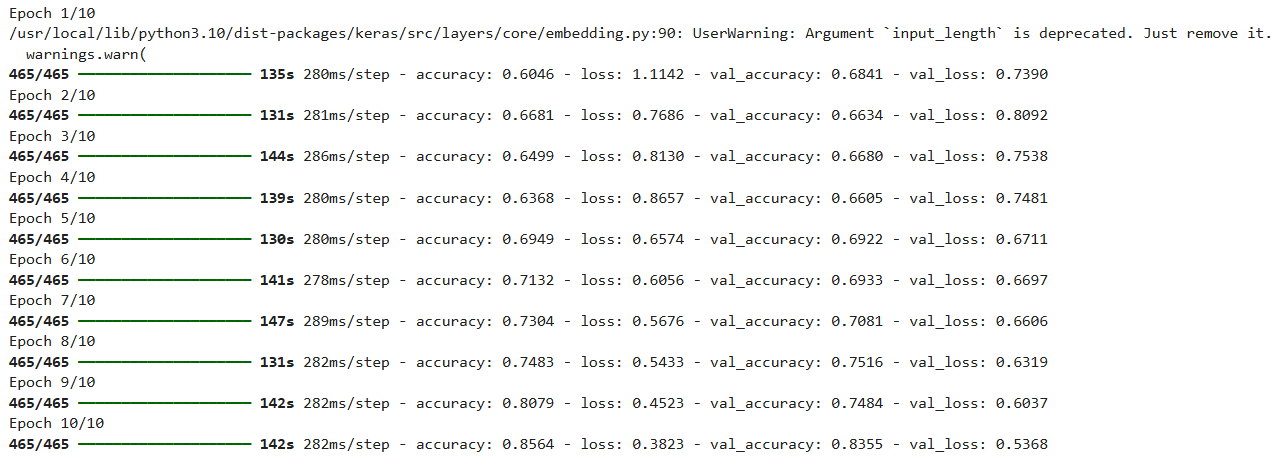
\includegraphics[width=1.0\textwidth]{Images/LSTM Epoch.png}  
    \caption{Output for LSTM Epochs}
    \label{LSTm Epochs}  % Label for referencing the figure
\end{figure}

\begin{figure}[h!]  
    \centering
    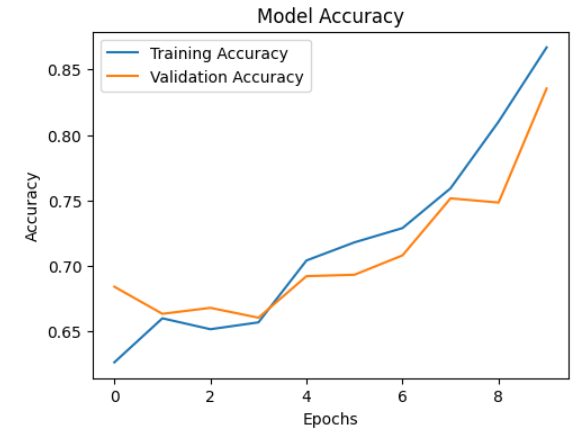
\includegraphics[width=0.85\textwidth]{Images/LSTM Accuracy v Epoch.png}  
    \caption{Accuracy v/s Epoch}
    \label{Accuracy vs Epoch LSTM}  % Label for referencing the figure
\end{figure}

\begin{figure}[h!]  
    \centering
    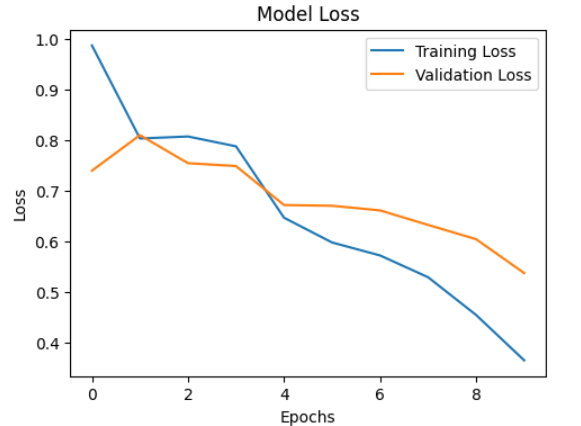
\includegraphics[width=0.85\textwidth]{Images/LSTM Loss v Epoch.png}  
    \caption{Loss v/s Epoch}
    \label{Loss vs Epoch LSTM}  % Label for referencing the figure
\end{figure}


\subsubsection{Hyperparamter Tuning Using RandomizedSearchCV}

\begin{tcolorbox}[colback=gray!5!white, colframe=gray!80!black, boxrule=0.5pt, title=Logistic Regression]
\begin{lstlisting}[language=Python]
import pandas as pd
from sklearn.model_selection import train_test_split, RandomizedSearchCV
from sklearn.feature_extraction.text import CountVectorizer
from sklearn.linear_model import LogisticRegression
from sklearn.metrics import accuracy_score, classification_report

# Load the preprocessed dataset
dataset = pd.read_csv('preprocessed_mental_health.csv')

# Check if 'cleaned_text' and 'mental_health_issue' columns exist
if 'cleaned_text' not in dataset.columns or 'mental_health_issue' not in dataset.columns:
    raise ValueError("The dataset must have 'cleaned_text' and 'mental_health_issue' columns.")
\end{lstlisting}
\end{tcolorbox}

\begin{tcolorbox}[colback=gray!5!white, colframe=gray!80!black, boxrule=0.5pt, title=Logistic Regression]
    \begin{lstlisting}[language=Python]
# Remove rows with missing values in 'cleaned_text' column
dataset.dropna(subset=['cleaned_text'], inplace=True)

# Initialize the CountVectorizer and fit/transform the cleaned text
HPLRvectorizer = CountVectorizer()
X = HPLRvectorizer.fit_transform(dataset['cleaned_text'])

# Prepare the target variable
y = dataset['mental_health_issue']

# Split the dataset into Training and Test Sets
X_train, X_test, y_train, y_test = train_test_split(X, y, test_size=0.2, random_state=42)

# Initialize the Logistic Regression model
HPLRmodel = LogisticRegression(max_iter=200)

# Define the hyperparameter grid for Randomized Search
param_distributions = {
    'C': [0.001, 0.01, 0.1, 1, 10, 100],       # Inverse of regularization strength
    'penalty': ['l1', 'l2', 'elasticnet', 'none'],  # Regularization types
    'solver': ['liblinear', 'saga']             # Solvers that support l1, elasticnet
}

# Initialize RandomizedSearchCV
random_search = RandomizedSearchCV(estimator=HPLRmodel, param_distributions=param_distributions,
                                   n_iter=10, scoring='accuracy', cv=5, n_jobs=-1, random_state=42)

# Fit RandomizedSearchCV
random_search.fit(X_train, y_train)

# Best hyperparameters from Random Search
print("Best Hyperparameters:", random_search.best_params_)

# Best model from Random Search
best_modelLR = random_search.best_estimator_

# Make predictions using the best model
y_pred = best_modelLR.predict(X_test)

\end{lstlisting}
\end{tcolorbox}

\begin{tcolorbox}[colback=gray!5!white, colframe=gray!80!black, boxrule=0.5pt, title=Logistic Regression]
    \begin{lstlisting}[language=Python]
# Evaluate the model
accuracy = accuracy_score(y_test, y_pred)
print(f'Accuracy: {accuracy * 100:.2f}%')

# Print classification report
print("Classification Report:\n", classification_report(y_test, y_pred))
\end{lstlisting}
\end{tcolorbox}

\noindent
The above code demonstrates a machine learning workflow for classifying mental health issues using \texttt{LogisticRegression} with hyperparameter tuning. The dataset is loaded using \texttt{pandas}, and a check ensures the presence of \texttt{'cleaned\_text'} and \texttt{'mental\_health\_issue'} columns. Missing values in \texttt{'cleaned\_text'} are dropped to prevent processing errors. The textual data is transformed into a numerical format using \texttt{CountVectorizer}, which converts text into a bag-of-words representation. The dataset is then split into training and testing sets using \texttt{train\_test\_split}. A logistic regression model is initialized, and the hyperparameter grid is defined, including parameters like \texttt{C} (inverse of regularization strength), \texttt{penalty}, and \texttt{solver}. Hyperparameter tuning is performed using \texttt{RandomizedSearchCV}, which searches for the best model configuration by sampling parameter combinations. The best model is used to make predictions on the test set, and evaluation metrics such as accuracy and a classification report are printed. This approach ensures optimal model performance and generalization to new data.

\begin{tcolorbox}[colback=gray!5!white, colframe=gray!80!black, boxrule=0.5pt, title=K Nearest Neighbours]
    \begin{lstlisting}[language=Python]
import pandas as pd
from sklearn.model_selection import train_test_split, RandomizedSearchCV
from sklearn.feature_extraction.text import CountVectorizer
from sklearn.neighbors import KNeighborsClassifier
from sklearn.metrics import accuracy_score, classification_report, confusion_matrix

# Load the preprocessed dataset
dataset = pd.read_csv('preprocessed_mental_health.csv')
# Check if 'cleaned_text' and 'mental_health_issue' columns exist
if 'cleaned_text' not in dataset.columns or 'mental_health_issue' not in dataset.columns:
    raise ValueError("The dataset must have 'cleaned_text' and 'mental_health_issue' columns.")
\end{lstlisting}
\end{tcolorbox}

\begin{tcolorbox}[colback=gray!5!white, colframe=gray!80!black, boxrule=0.5pt, title=K Nearest Neighbours]
    \begin{lstlisting}[language=Python]
# Remove rows with missing values in 'cleaned_text' column
dataset.dropna(subset=['cleaned_text'], inplace=True)

# Initialize the CountVectorizer and fit/transform the cleaned text
HPTKNNvectorizer = CountVectorizer()
X = HPTKNNvectorizer.fit_transform(dataset['cleaned_text'])

# Prepare the target variable
y = dataset['mental_health_issue']

# Split the dataset into Training and Test Sets
X_train, X_test, y_train, y_test = train_test_split(X, y, test_size=0.2, random_state=42)

# Initialize the k-NN classifier
knn = KNeighborsClassifier()

# Define the hyperparameter grid for Randomized Search
param_distributions = {
    'n_neighbors': [3, 4, 5, 6, 7, 8, 9, 10, 11, 12, 13, 15, 14, 15, 16, 17, 18, 19, 20],
        # Different values for number of neighbors
    'metric': ['euclidean', 'manhattan', 'chebyshev', 'minkowski'],  # Different distance metrics
    'weights': ['uniform', 'distance']  # Weighing options for neighbors
}

# Initialize RandomizedSearchCV
random_search = RandomizedSearchCV(estimator=knn, param_distributions=param_distributions,
                                    n_iter=10, scoring='accuracy', cv=5, n_jobs=-1, random_state=42)

# Fit RandomizedSearchCV
random_search.fit(X_train, y_train)

# Best hyperparameters from Random Search
print("Best Hyperparameters:", random_search.best_params_)

# Best model from Random Search
best_knn = random_search.best_estimator_

# Make predictions using the best model
y_pred = best_knn.predict(X_test)
\end{lstlisting}
\end{tcolorbox}

\begin{tcolorbox}[colback=gray!5!white, colframe=gray!80!black, boxrule=0.5pt, title=K Nearest Neighbours]
    \begin{lstlisting}[language=Python]
# Evaluate the model
accuracy = accuracy_score(y_test, y_pred)
print(f'Accuracy: {accuracy * 100:.2f}%')

# Print classification report
print("Classification Report:\n", classification_report(y_test, y_pred))

# Print confusion matrix
print("Confusion Matrix:\n", confusion_matrix(y_test, y_pred))
    \end{lstlisting}
\end{tcolorbox}

\noindent
This code implements a k-Nearest Neighbors (k-NN) classifier for classifying mental health issues from text data using hyperparameter tuning via RandomizedSearchCV. First, it loads a preprocessed dataset, ensuring the existence of critical columns, \texttt{cleaned\_text} (features) and \texttt{mental\_health\_issue} (target). Rows with missing values in the \texttt{cleaned\_text} column are removed to maintain data integrity. The text is vectorized into numerical format using \texttt{CountVectorizer}, converting text into a bag-of-words model. The features (\(X\)) and target (\(y\)) are split into training (80\%) and test (20\%) datasets to ensure proper model evaluation. The k-NN model is initialized without predefined parameters, and a hyperparameter grid is defined for tuning. This grid explores various values for the number of neighbors (\texttt{n\_neighbors}), distance metrics (\texttt{metric}), and neighbor weighting options (\texttt{weights}). \texttt{RandomizedSearchCV} is then used to optimize these parameters by training multiple k-NN models with combinations from the grid, evaluating them with 5-fold cross-validation, and scoring based on accuracy. The best combination of hyperparameters is identified and used to configure the final k-NN model. The model is then tested on unseen data (test set), and its performance is evaluated by calculating the accuracy, a classification report detailing precision, recall, F1-score for each class, and a confusion matrix showing true vs. predicted classifications. This approach balances computational efficiency with robustness, enabling the selection of an optimized k-NN model for mental health classification.


\begin{tcolorbox}[colback=gray!5!white, colframe=gray!80!black, boxrule=0.5pt, title=Support Vector Machine]
    \begin{lstlisting}[language=Python]
import pandas as pd
from sklearn.model_selection import train_test_split, RandomizedSearchCV
from sklearn.feature_extraction.text import CountVectorizer
from sklearn.svm import SVC
from sklearn.metrics import accuracy_score, classification_report
\end{lstlisting}
\end{tcolorbox}

\begin{tcolorbox}[colback=gray!5!white, colframe=gray!80!black, boxrule=0.5pt, title=Support Vector Machine]
    \begin{lstlisting}[language=Python]
# Load the preprocessed dataset
dataset = pd.read_csv('preprocessed_mental_health.csv')

# Check if 'cleaned_text' and 'mental_health_issue' columns exist
if 'cleaned_text' not in dataset.columns or 'mental_health_issue' not in dataset.columns:
    raise ValueError("The dataset must have 'cleaned_text' and 'mental_health_issue' columns.")

# Remove rows with missing values in 'cleaned_text' column
dataset.dropna(subset=['cleaned_text'], inplace=True)

# Initialize the CountVectorizer and fit/transform the cleaned text
vectorizer = CountVectorizer()
X = vectorizer.fit_transform(dataset['cleaned_text'])

# Prepare the target variable
y = dataset['mental_health_issue']

# Split the dataset into Training and Test Sets
X_train, X_test, y_train, y_test = train_test_split(X, y, test_size=0.2, random_state=42)

# Initialize the SVC model
model = SVC()

# Define the hyperparameter grid for Randomized Search
param_distributions = {
    'C': [0.1, 1, 10, 100],               # Regularization parameter
    'kernel': ['linear', 'rbf', 'poly'],  # Kernel types
    'gamma': ['scale', 'auto', 0.1, 1],   # Kernel coefficient for 'rbf', 'poly', and 'sigmoid'
}

# Initialize RandomizedSearchCV
random_search = RandomizedSearchCV(estimator=model, param_distributions=param_distributions,
                                    n_iter=10, scoring='accuracy', cv=5, n_jobs=-1, random_state=42)

# Fit RandomizedSearchCV
random_search.fit(X_train, y_train)
\end{lstlisting}
\end{tcolorbox}

\begin{tcolorbox}[colback=gray!5!white, colframe=gray!80!black, boxrule=0.5pt, title=Support Vector Machine]
    \begin{lstlisting}[language=Python]
# Best hyperparameters from Random Search
print("Best Hyperparameters:", random_search.best_params_)

# Best model from Random Search
best_model = random_search.best_estimator_

# Make predictions using the best model
y_pred = best_model.predict(X_test)

# Evaluate the model
accuracy = accuracy_score(y_test, y_pred)
print(f'Accuracy: {accuracy * 100:.2f}%')

# Print classification report
print("Classification Report:\n", classification_report(y_test, y_pred))
\end{lstlisting}
\end{tcolorbox}

\noindent
This code implements a Support Vector Classifier (SVC) for classifying mental health issues from text data using hyperparameter tuning via RandomizedSearchCV. It begins by loading a preprocessed dataset and ensuring that essential columns, \texttt{cleaned\_text} (features) and \texttt{mental\_health\_issue} (target), are present. Any rows with missing values in the \texttt{cleaned\_text} column are removed to ensure clean data. The text is then vectorized into a numerical format using \texttt{CountVectorizer}, transforming it into a bag-of-words representation. The features (\(X\)) and target (\(y\)) are split into training (80\%) and test (20\%) sets for model validation. The SVC model is initialized without predefined hyperparameters, and a hyperparameter grid is defined for tuning. This grid includes different values for the regularization parameter (\texttt{C}), kernel types (\texttt{kernel}), and the kernel coefficient (\texttt{gamma}). \texttt{RandomizedSearchCV} is employed to find the best combination of these parameters by evaluating multiple models with various hyperparameter combinations through 5-fold cross-validation, using accuracy as the scoring metric. The best set of hyperparameters is selected to configure the final SVC model. The model is then evaluated on the test set by making predictions, and its performance is measured by calculating the accuracy, as well as generating a classification report that includes precision, recall, and F1-score for each class. This approach ensures the selection of the most optimized SVC model for the classification of mental health issues from text data.

\begin{tcolorbox}[colback=gray!5!white, colframe=gray!80!black, boxrule=0.5pt, title=Naive Bayes]
    \begin{lstlisting}[language=Python]
import pandas as pd
from sklearn.model_selection import train_test_split, RandomizedSearchCV
from sklearn.feature_extraction.text import CountVectorizer
from sklearn.naive_bayes import MultinomialNB
from sklearn.metrics import accuracy_score, classification_report, confusion_matrix
from scipy.stats import uniform

# Load the preprocessed dataset
dataset = pd.read_csv('preprocessed_mental_health.csv')

# Check if 'cleaned_text' and 'mental_health_issue' columns exist
if 'cleaned_text' not in dataset.columns or 'mental_health_issue' not in dataset.columns:
    raise ValueError("The dataset must have 'cleaned_text' and 'mental_health_issue' columns.")

# Remove rows with missing values in 'cleaned_text' column
dataset.dropna(subset=['cleaned_text'], inplace=True)

# Initialize the CountVectorizer and fit/transform the cleaned text
vectorizer = CountVectorizer()
X = vectorizer.fit_transform(dataset['cleaned_text'])

# Prepare the target variable
y = dataset['mental_health_issue']

# Split the dataset into Training and Test Sets
X_train, X_test, y_train, y_test = train_test_split(X, y, test_size=0.2, random_state=42)

# Initialize the Naive Bayes model
naive_bayes_model = MultinomialNB()

# Define the parameter distribution for Randomized Search
param_distributions = {
    'alpha': uniform(0.001, 5.0)  # Sampling alpha from a uniform distribution
}
\end{lstlisting}
\end{tcolorbox}

\begin{tcolorbox}[colback=gray!5!white, colframe=gray!80!black, boxrule=0.5pt, title=Naive Bayes]
    \begin{lstlisting}[language=Python]
# Initialize RandomizedSearchCV
random_search = RandomizedSearchCV(estimator=naive_bayes_model, param_distributions=param_distributions,
                                    n_iter=10, scoring='accuracy', cv=5, n_jobs=-1, random_state=42)

# Fit RandomizedSearchCV
random_search.fit(X_train, y_train)

# Best hyperparameters from Random Search
print("Best Hyperparameters:", random_search.best_params_)

# Best model from Random Search
best_model = random_search.best_estimator_

# Make predictions using the best model
y_pred = best_model.predict(X_test)

# Evaluate the model
accuracy = accuracy_score(y_test, y_pred)
print(f'Accuracy: {accuracy * 100:.2f}%')

# Print classification report
print("Classification Report:\n", classification_report(y_test, y_pred))

# Print confusion matrix
print("Confusion Matrix:\n", confusion_matrix(y_test, y_pred))        
    \end{lstlisting}
\end{tcolorbox}

\noindent
This code implements a Naive Bayes classifier using the MultinomialNB algorithm to classify mental health issues from text data, with hyperparameter tuning via RandomizedSearchCV. The dataset is first loaded, ensuring the required columns, \texttt{cleaned\_text} (features) and \texttt{mental\_health\_issue} (target), exist. Rows with missing values in the \texttt{cleaned\_text} column are removed to maintain data quality. The text is vectorized using \texttt{CountVectorizer}, converting it into a bag-of-words representation. The features (\(X\)) and target (\(y\)) are then split into training (80\%) and test (20\%) sets to facilitate proper evaluation. The Naive Bayes model is initialized, and a parameter distribution for \texttt{alpha} is defined using a uniform distribution, sampling values between 0.001 and 5.0. \texttt{RandomizedSearchCV} is utilized to explore different values for \texttt{alpha} over 10 iterations, using 5-fold cross-validation and accuracy as the scoring metric. The best hyperparameters are identified and used to configure the final Naive Bayes model. The model is then tested on the unseen data (test set).


\subsubsection{Ensemble Model with Logistic Regression and XGBoost}

\begin{tcolorbox}[colback=gray!5!white, colframe=gray!80!black, boxrule=0.5pt, title=Model Loading and Preprocessing]
    \begin{lstlisting}[language=Python]
import pickle
from sklearn.ensemble import StackingClassifier
from sklearn.linear_model import LogisticRegression
from sklearn.metrics import accuracy_score, classification_report
import xgboost as xgb
import pandas as pd

# Load the Logistic Regression model and vectorizer
with open('LRmodel.pkl', 'rb') as file:
    lr_model = pickle.load(file)

with open('LRvectorizer.pkl', 'rb') as file:
    lr_vectorizer = pickle.load(file)

# Load the XGBoost model, label encoder, and TF-IDF vectorizer
with open('xgb_model.pkl', 'rb') as file:
    xgb_model = pickle.load(file)

with open('label_encoder.pkl', 'rb') as file:
    label_encoder = pickle.load(file)

with open('tfidf_vectorizer.pkl', 'rb') as file:
    tfidf_vectorizer = pickle.load(file)
    \end{lstlisting}
\end{tcolorbox}

\noindent
This Python code is centered around preparing a machine learning workflow by loading pre-trained models and their corresponding preprocessing tools. It begins by importing essential libraries for model evaluation and stacking. The \texttt{pickle} library is specifically used to load serialized Python objects, enabling the restoration of previously trained models and utilities saved as \texttt{.pkl} files. The first part of the code loads a Logistic Regression model along with its associated vectorizer. The Logistic Regression model is deserialized from the \texttt{LRmodel.pkl} file, which represents a trained model capable of predicting outcomes based on vectorized text data. The corresponding vectorizer, stored in \texttt{LRvectorizer.pkl}, is also loaded. This vectorizer, likely a \texttt{CountVectorizer}, converts raw text into numerical feature vectors, which serve as the input for the Logistic Regression model. By loading these components, the workflow ensures consistency with the preprocessing and modeling steps used during training. In the next section, the code loads an XGBoost model alongside its associated tools. The XGBoost model is deserialized from \texttt{xgb\_model.pkl} and represents another trained model designed to classify text data. To facilitate this, the code also loads a label encoder from \texttt{label\_encoder.pkl}. The label encoder is responsible for mapping textual class labels (e.g., "depression" or "normal") to numerical values required by machine learning models. Furthermore, the \texttt{tfidf\_vectorizer.pkl} is loaded to preprocess text data using the Term Frequency-Inverse Document Frequency (TF-IDF) approach, which captures the importance of words in a document relative to a corpus. This ensures that the input text is transformed in a manner consistent with the original training setup of the XGBoost model. The design of this code emphasizes efficiency and consistency by leveraging pre-trained components. Instead of retraining models, it restores them from their serialized forms, enabling immediate use for predictions or integration into ensemble learning setups. This approach also ensures that text preprocessing remains identical to the training phase, avoiding discrepancies in input data handling. By combining these tools, the foundation is laid for complex tasks such as making predictions or building advanced models like stacked classifiers.

\begin{tcolorbox}[colback=gray!5!white, colframe=gray!80!black, boxrule=0.5pt, title=Data Preparation]
\begin{lstlisting}[language=Python]
# Load the test dataset
data = pd.read_csv('preprocessed_mental_health.csv')

# Check if 'cleaned_text' column exists
if 'cleaned_text' not in data.columns:
    raise ValueError("The dataset must have a 'cleaned_text' column.")

# Remove rows with missing values in 'cleaned_text'
data.dropna(subset=['cleaned_text'], inplace=True)

# Split features and target
X_test = data['cleaned_text']
y_test = data['mental_health_issue']

# Encode target labels
y_test = label_encoder.transform(y_test)

# Transform the text using the respective vectorizers
X_test_lr = lr_vectorizer.transform(X_test)  # Logistic Regression vectorizer
X_test_xgb = tfidf_vectorizer.transform(X_test)  # XGBoost vectorizer
\end{lstlisting}
\end{tcolorbox}
    
\noindent
This code snippet focuses on preparing the test dataset for evaluation with pre-trained machine learning models, specifically Logistic Regression and XGBoost. First, the test dataset is loaded from a CSV file named \texttt{preprocessed\_mental\_health.csv} using \texttt{pd.read\_csv}. The dataset is expected to have been preprocessed earlier, containing features and corresponding labels. The code then checks for the existence of a critical column named \texttt{cleaned\_text}. If this column is missing, a \texttt{ValueError} is raised, ensuring that the dataset meets the required format for subsequent steps. Next, the code removes rows with missing values in the \texttt{cleaned\_text} column using \texttt{data.dropna}. This step ensures the dataset is clean and free of incomplete rows that could potentially cause errors during text transformation or model evaluation. After this cleaning process, the dataset is split into features (\texttt{X\_test}) and target labels (\texttt{y\_test}). The features contain the preprocessed text, while the target labels represent the mental health issues corresponding to each text entry. The target labels in \texttt{y\_test} are then encoded into numerical format using a preloaded \texttt{label\_encoder}. This encoding is crucial because machine learning models require numerical representations of categorical labels for classification tasks. By transforming the labels to integers, the encoded labels are consistent with the classes used during the model's training phase. Finally, the text data in \texttt{X\_test} is vectorized using two pre-trained vectorizers. The \texttt{lr\_vectorizer}, likely a \texttt{CountVectorizer} or similar, is applied to produce feature vectors suitable for the Logistic Regression model. Simultaneously, the \texttt{tfidf\_vectorizer} is applied to transform the same text data into feature vectors optimized for the XGBoost model. These transformations ensure that the test data aligns with the feature representations learned by the respective models during training. This setup allows for seamless evaluation of the Logistic Regression and XGBoost models on the same dataset, maintaining consistency with their training configurations.

\begin{tcolorbox}[colback=gray!5!white, colframe=gray!80!black, boxrule=0.5pt, title=Combine Base Model Predictions]
\begin{lstlisting}[language=Python]
import numpy as np

# Get predictions from the base models
lr_predictions_proba = lr_model.predict_proba(X_test_lr)
xgb_predictions_proba = xgb_model.predict_proba(X_test_xgb)

# Combine predictions as new features
stacked_features = np.hstack((lr_predictions_proba, xgb_predictions_proba))
\end{lstlisting}
\end{tcolorbox}

\noindent
This Python code demonstrates a fundamental step in stacking ensemble learning by combining the prediction probabilities of base models into a single feature set. The process begins with obtaining predictions from two pre-trained models: a Logistic Regression model (\texttt{lr\_model}) and an XGBoost model (\texttt{xgb\_model}). These models generate class probability distributions for the test dataset, which are then used as input features for a meta-learner in an ensemble framework. First, the code uses the \texttt{predict\_proba} method of each model to calculate the probabilities associated with each class for every test instance. For the Logistic Regression model, the feature set (\texttt{X\_test\_lr}) is passed to \texttt{lr\_model.predict\_proba}, producing a 2D array (\texttt{lr\_predictions\_proba}) where each row contains the class probabilities for a corresponding instance. Similarly, the XGBoost model processes its input features (\texttt{X\_test\_xgb}) to generate a comparable 2D array (\texttt{xgb\_predictions\_proba}) of class probabilities. Next, the code combines these probability arrays to form a new feature set, referred to as \texttt{stacked\_features}. This is accomplished using the \texttt{np.hstack} function from the NumPy library, which horizontally stacks the arrays column-wise. The resulting \texttt{stacked\_features} array contains concatenated probability distributions from both models for each instance. For example, if there are three classes and 100 instances, the combined feature set will have 100 rows and six columns (three from each model). This stacked feature set serves as input to a meta-learner, enabling it to make final predictions by leveraging the strengths of both base models. By integrating predictions in this manner, the stacking approach aims to improve classification performance by reducing errors associated with individual models. The meta-learner effectively learns how to optimally combine these predictions to produce more accurate outcomes.
    
\begin{tcolorbox}[colback=gray!5!white, colframe=gray!80!black, boxrule=0.5pt, title=Train Meta-Learner]
\begin{lstlisting}[language=Python]
# Train meta-learner using combined features (optional step if not pre-trained)
X_train_meta, y_train_meta = stacked_features, y_test  # Example using test data as meta-training data

meta_learner = LogisticRegression(max_iter=5000)
meta_learner.fit(X_train_meta, y_train_meta)

# Save the trained meta-learner
with open('meta_learner.pkl', 'wb') as file:
    pickle.dump(meta_learner, file)
\end{lstlisting}
\end{tcolorbox}

\noindent
This Python code focuses on training a meta-learner in the context of stacking ensemble learning. A meta-learner is a secondary machine learning model trained on the outputs of base models, with the goal of combining their predictions to achieve higher accuracy and robustness. The first step involves defining the training data for the meta-learner. The variable \texttt{X\_train\_meta} is set to the combined feature set (\texttt{stacked\_features}), which contains the concatenated prediction probabilities from base models like Logistic Regression and XGBoost. These features represent the likelihood of each class for every instance, as estimated by the base models. The variable \texttt{y\_train\_meta} holds the true labels (\texttt{y\_test}), which are used as the target variable for training the meta-learner. The code then initializes a Logistic Regression model as the meta-learner. The parameter \texttt{max\_iter=5000} ensures that the optimization process has sufficient iterations to converge, particularly for complex datasets or large feature sets. The \texttt{fit} method is called to train the meta-learner using the stacked features and corresponding labels. During this training process, the meta-learner learns how to optimally combine the prediction probabilities from the base models to produce more accurate final predictions. After training, the code saves the meta-learner to a file named \texttt{meta\_learner.pkl} using the \texttt{pickle.dump} function. This step serializes the trained model, enabling its reuse for future predictions without needing to retrain it. By saving the meta-learner, the workflow becomes more efficient, as the combined expertise of the base models and the meta-learner can be leveraged in subsequent tasks. This approach exemplifies the flexibility and power of stacking ensemble learning, where a meta-learner synthesizes the strengths of multiple base models to enhance predictive performance. The ability to save the meta-learner ensures that this improved model can be deployed in practical applications with minimal computational overhead.
    

\begin{tcolorbox}[colback=gray!5!white, colframe=gray!80!black, boxrule=0.5pt, title=Evaluate Meta-Learner and Ensemble Model]
\begin{lstlisting}[language=Python]
from sklearn.metrics import confusion_matrix

# Load the pre-trained meta-learner
with open('meta_learner.pkl', 'rb') as file:
    meta_learner = pickle.load(file)

# Predict using the meta-learner
final_predictions = meta_learner.predict(stacked_features)

# Evaluate the ensemble model
accuracy = accuracy_score(y_test, final_predictions)
report = classification_report(y_test, final_predictions, target_names=label_encoder.classes_)

print(f"Accuracy: {accuracy * 100:.2f}%")
print("Classification Report:\n", report)
# Print confusion matrix
print("Confusion Matrix:\n", confusion_matrix(y_test, final_predictions))
\end{lstlisting}
\end{tcolorbox}

\noindent
This Python code evaluates the performance of a stacking ensemble model, specifically focusing on the meta-learner. The workflow begins by loading the pre-trained meta-learner from a file named \texttt{meta\_learner.pkl}. Using the \texttt{pickle.load} function, the serialized meta-learner model is deserialized and prepared for making predictions. The next step involves generating predictions with the meta-learner. The model uses the stacked features, which are the combined prediction probabilities from the base models (e.g., Logistic Regression and XGBoost). The \texttt{predict} method of the meta-learner outputs the final predicted labels for the test data. To evaluate the ensemble model's effectiveness, the code computes its accuracy using the \texttt{accuracy\_score} function. Accuracy is expressed as the percentage of correctly classified instances relative to the total instances in the test set. Additionally, the \texttt{classification\_report} function is used to generate a detailed performance summary. This report includes precision, recall, F1-score, and support for each mental health class. The \texttt{target\_names} parameter ensures that the report associates the predicted numerical labels with their corresponding class names, as encoded by the label encoder. The evaluation also involves generating a confusion matrix, which provides an in-depth view of the classification performance. The \texttt{confusion\_matrix} function compares the true labels (\texttt{y\_test}) with the predicted labels (\texttt{final\_predictions}), resulting in a matrix that shows the counts of true positives, true negatives, false positives, and false negatives for each class. Finally, the accuracy, classification report, and confusion matrix are printed to the console. This comprehensive evaluation allows the user to assess the ensemble model's overall performance, identify any weaknesses (e.g., misclassifications for specific classes), and confirm the effectiveness of the meta-learner in combining predictions from base models. This structured approach to evaluation underscores the advantages of stacking ensemble learning, demonstrating how the combined insights from multiple base models and a meta-learner can lead to robust predictions and meaningful performance metrics.

\vspace{1em}

\noindent
In ensemble learning, combining different models like Logistic Regression and XGBoost often leads to improved results due to their complementary strengths. Logistic Regression, being a linear model, excels in problems where the relationship between features is linear. It is simple, interpretable, and computationally efficient, making it effective for text-based classification tasks when the relationship between the features (such as word counts or TF-IDF scores) and the target variable is linear. However, Logistic Regression has some limitations: it struggles with capturing complex non-linear relationships and can perform poorly when the data is highly imbalanced or when there are interactions between features that the model cannot capture. On the other hand, XGBoost (Extreme Gradient Boosting) is a powerful tree-based model that can capture complex, non-linear relationships and interactions between features, making it particularly effective for handling large, noisy, and high-dimensional datasets like text. It builds an ensemble of decision trees and iteratively improves the model by minimizing errors. However, XGBoost also has its drawbacks. It requires careful tuning of hyperparameters (e.g., learning rate, number of trees, and tree depth) and can be computationally expensive, especially for large datasets. Additionally, while it can model non-linear relationships well, it lacks the interpretability of simpler models like Logistic Regression. By combining Logistic Regression and XGBoost in an ensemble learning setup, the two models can complement each other. Logistic Regression can provide a robust baseline when the relationships between features are linear, while XGBoost can enhance the model's ability to capture more complex patterns. This hybrid approach leverages the strengths of both models—Logistic Regression's simplicity and speed, alongside XGBoost's power in modeling complex interactions.




% ------------------------- Implementation Ends -----------------------------
